\documentclass[tikz,border=5pt]{standalone}
\usepackage[T1]{fontenc}
\usepackage{lmodern,amsmath,amssymb}
\usetikzlibrary{arrows.meta,calc,positioning,fit,backgrounds,shapes.geometric,matrix,decorations.pathreplacing,patterns}
\definecolor{ink}{gray}{0.08}
\definecolor{wash}{gray}{0.965}
\definecolor{soft}{gray}{0.45}
\tikzset{box/.style={draw=ink,line width=.65pt,fill=white,align=center,inner sep=4pt,outer sep=0pt,font=\small},flow/.style={draw=ink,line width=.65pt,-{Latex[length=1.8mm,width=1.3mm]},rounded corners=2pt},annotation/.style={font=\scriptsize,text=soft,align=center},groupbox/.style={draw=soft,dashed,line width=.45pt,fill=wash}}
\begin{document}
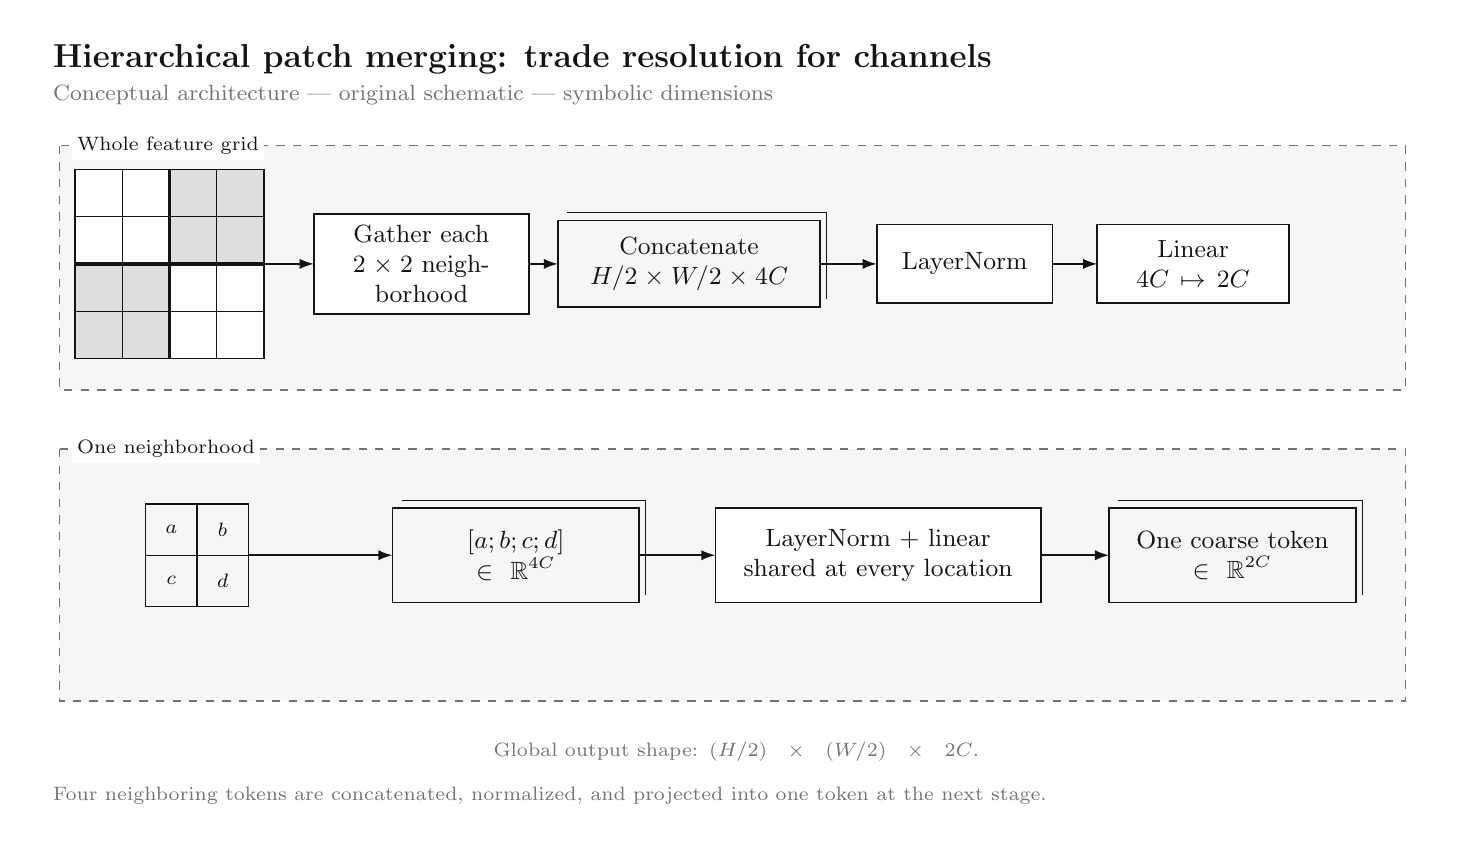
\begin{tikzpicture}[x=1cm,y=-1cm,font=\rmfamily,text=ink]

\path[use as bounding box] (0,0) rectangle (18,10);
\node[anchor=west,font=\large\bfseries] at (.2,.4) {Hierarchical patch merging: trade resolution for channels};
\node[anchor=west,font=\footnotesize,text=soft] at (.2,.85) {Conceptual architecture | original schematic | symbolic dimensions};
\begin{pgfonlayer}{background}
\draw[groupbox] (0.4,1.5) rectangle (17.5,4.6);
\node[anchor=west,font=\scriptsize,fill=white,inner sep=2pt] at (0.55,1.5) {Whole feature grid};
\draw[groupbox] (0.4,5.35) rectangle (17.5,8.55);
\node[anchor=west,font=\scriptsize,fill=white,inner sep=2pt] at (0.55,5.35) {One neighborhood};
\end{pgfonlayer}
\node[align=center,inner sep=0pt,outer sep=0pt,font=\small,minimum width=2.4cm,minimum height=2.0cm,text width=2.15cm] (input) at (1.8,3.0) {};
\node[box,minimum width=2.7cm,minimum height=1.1cm,text width=2.45cm] (gather) at (5.0,3.0) {Gather each\\$2\times2$ neighborhood};
\node[box,fill=wash,minimum width=3.3cm,minimum height=1.1cm,text width=3.05cm] (concat) at (8.4,3.0) {Concatenate\\$H/2\times W/2\times4C$};
\draw[ink,line width=.4pt] (6.85,2.35) -- (10.15,2.35) -- (10.15,3.4499999999999997);
\node[box,minimum width=2.2cm,minimum height=1.0cm,text width=1.9500000000000002cm] (norm) at (11.9,3.0) {LayerNorm};
\node[box,minimum width=2.4cm,minimum height=1.0cm,text width=2.15cm] (linear) at (14.8,3.0) {Linear\\$4C\mapsto2C$};
\node[align=center,inner sep=0pt,outer sep=0pt,font=\small,minimum width=1.3cm,minimum height=1.3cm,text width=1.05cm] (local) at (2.15,6.7) {};
\node[box,fill=wash,minimum width=3.1cm,minimum height=1.2cm,text width=2.85cm] (vec) at (6.2,6.7) {$[a;b;c;d]$\\$\in\mathbb R^{4C}$};
\draw[ink,line width=.4pt] (4.75,6.000000000000001) -- (7.85,6.000000000000001) -- (7.85,7.2);
\node[box,minimum width=4.1cm,minimum height=1.2cm,text width=3.8499999999999996cm] (map) at (10.8,6.7) {LayerNorm + linear\\shared at every location};
\node[box,fill=wash,minimum width=3.1cm,minimum height=1.2cm,text width=2.85cm] (out) at (15.3,6.7) {One coarse token\\$\in\mathbb R^{2C}$};
\draw[ink,line width=.4pt] (13.85,6.000000000000001) -- (16.950000000000003,6.000000000000001) -- (16.950000000000003,7.2);
\begin{pgfonlayer}{background}
\draw[flow] (input.east) -- (gather.west);
\draw[flow] (gather.east) -- (concat.west);
\draw[flow] (concat.east) -- (norm.west);
\draw[flow] (norm.east) -- (linear.west);
\draw[flow] (local.east) -- (vec.west);
\draw[flow] (vec.east) -- (map.west);
\draw[flow] (map.east) -- (out.west);
\end{pgfonlayer}
\fill[black!0] (0.6,1.8) rectangle (1.2,2.4);
\fill[black!0] (1.2,1.8) rectangle (1.7999999999999998,2.4);
\fill[black!13] (1.7999999999999998,1.8) rectangle (2.4,2.4);
\fill[black!13] (2.4,1.8) rectangle (3.0,2.4);
\fill[black!0] (0.6,2.4) rectangle (1.2,3.0);
\fill[black!0] (1.2,2.4) rectangle (1.7999999999999998,3.0);
\fill[black!13] (1.7999999999999998,2.4) rectangle (2.4,3.0);
\fill[black!13] (2.4,2.4) rectangle (3.0,3.0);
\fill[black!13] (0.6,3.0) rectangle (1.2,3.5999999999999996);
\fill[black!13] (1.2,3.0) rectangle (1.7999999999999998,3.5999999999999996);
\fill[black!0] (1.7999999999999998,3.0) rectangle (2.4,3.5999999999999996);
\fill[black!0] (2.4,3.0) rectangle (3.0,3.5999999999999996);
\fill[black!13] (0.6,3.5999999999999996) rectangle (1.2,4.2);
\fill[black!13] (1.2,3.5999999999999996) rectangle (1.7999999999999998,4.2);
\fill[black!0] (1.7999999999999998,3.5999999999999996) rectangle (2.4,4.2);
\fill[black!0] (2.4,3.5999999999999996) rectangle (3.0,4.2);
\draw[ink,line width=.45pt] (0.6,1.8) rectangle (3.0,4.2);
\draw[ink,line width=.45pt] (1.2,1.8) -- (1.2,4.2);
\draw[ink,line width=.45pt] (1.7999999999999998,1.8) -- (1.7999999999999998,4.2);
\draw[ink,line width=.45pt] (2.4,1.8) -- (2.4,4.2);
\draw[ink,line width=.45pt] (0.6,2.4) -- (3.0,2.4);
\draw[ink,line width=.45pt] (0.6,3.0) -- (3.0,3.0);
\draw[ink,line width=.45pt] (0.6,3.5999999999999996) -- (3.0,3.5999999999999996);
\draw[ink,line width=1.25pt] (1.7999999999999998,1.8) -- (1.7999999999999998,4.2);
\draw[ink,line width=1.25pt] (0.6,3.0) -- (3.0,3.0);
\draw[ink,line width=.45pt] (1.5,6.05) rectangle (2.8,7.35);
\draw[ink,line width=.45pt] (2.15,6.05) -- (2.15,7.35);
\draw[ink,line width=.45pt] (1.5,6.7) -- (2.8,6.7);
\node[font=\scriptsize] at (1.825,6.375) {$a$};
\node[font=\scriptsize] at (2.475,6.375) {$b$};
\node[font=\scriptsize] at (1.825,7.025) {$c$};
\node[font=\scriptsize] at (2.475,7.025) {$d$};
\node[annotation,text width=13cm] at (9,9.2) {Global output shape: $(H/2)\times(W/2)\times2C$.};
\node[anchor=west,align=left,font=\scriptsize,text=soft,text width=17.6cm] at (.2,9.75) {Four neighboring tokens are concatenated, normalized, and projected into one token at the next stage.};
\end{tikzpicture}
\end{document}
